\documentclass[a4paper]{article}

\usepackage[utf8]{inputenc}
\usepackage{graphicx}
\usepackage{float}
\usepackage{amsmath}
\usepackage{indentfirst}
\usepackage{hyperref}
\usepackage[margin=2.8cm]{geometry}

\title{Workflow documentation}
\author{Gustave Li}
\date{Last updated: July 2021}

\begin{document}

\maketitle

\section{Introduction}
The Carotenoid-Porphyrin-\(\text{C}_{60}\) (\(\text{CPC}_{60}\)) triad molecule consists of a porphyrin covalently linked with a carotenoid and a \(\text{C}_{60}\) molecule (Figure~\ref{fig:CPC60}). Carotenoid is the excited-state electron donor and the \(\text{C}_{60}\) serves as the electron acceptor, while porphyrin acts as a bridge to separate the two parts and transfer electrons. The molecule is a mimicry of the natural photosynthetic center which utilize photons to initiate a complex series of electronic transitions to achieve a high-energy charge separated state. It absorbs UV visible light and produces a charge separated state (\(\text{CT}_{2}\)) where an electron is transferred from C to \(\text{C}_{60}\), producing a large dipole moment of 150 D. Due to its outstanding performance in photoinduced charge transfer, it has a great potential in organic solar cells.

\begin{figure}[H]
    \centering
    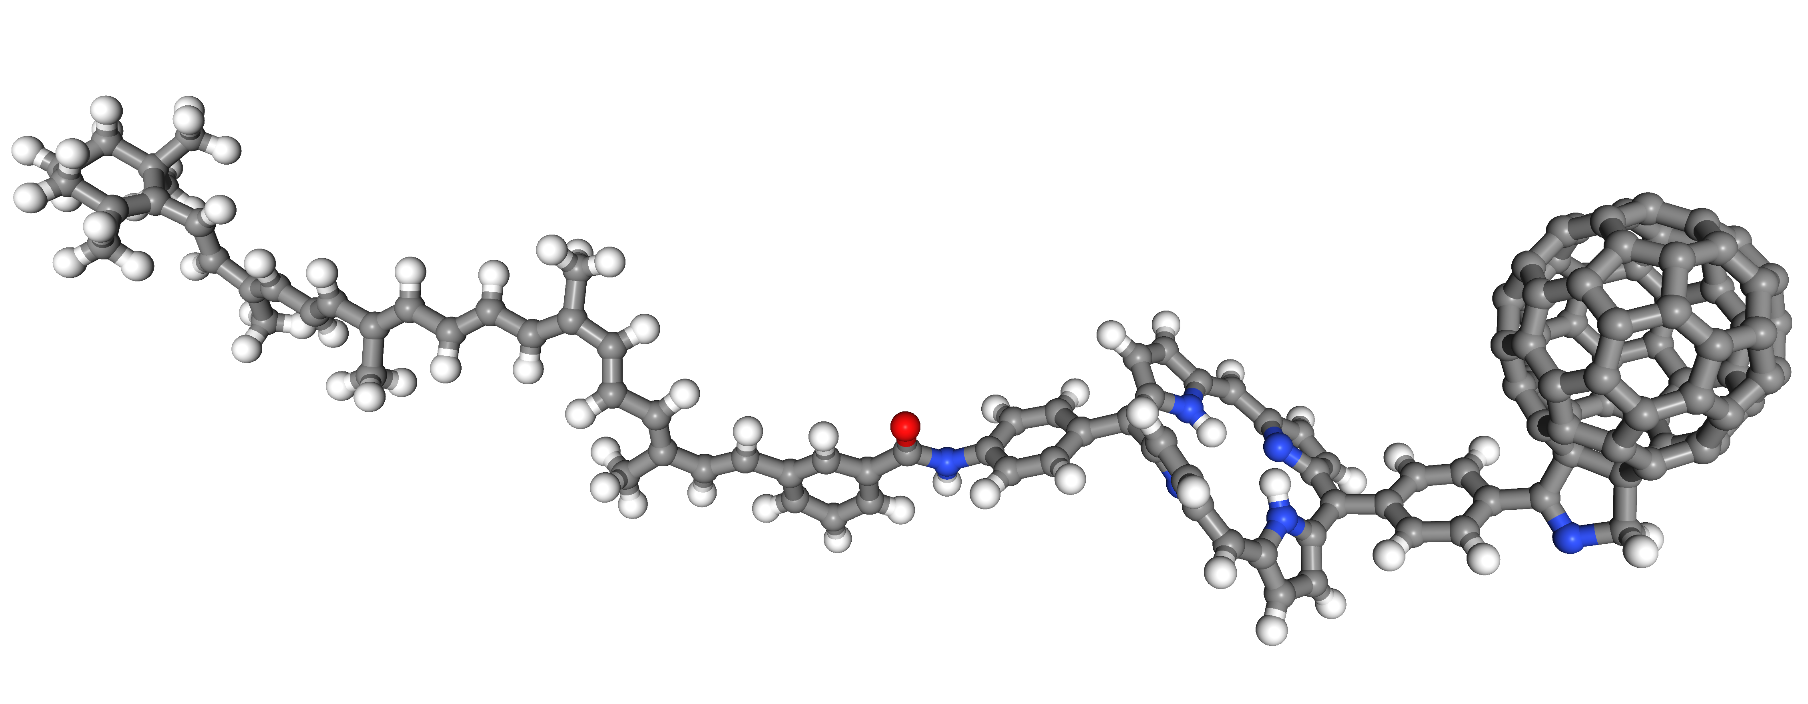
\includegraphics[width=0.75\linewidth]{projects/Gustave_Li/Docs/Triad.png}
    \caption{The \(\text{CPC}_{60}\) molecule}
    \label{fig:CPC60}
\end{figure}

However, Manna et al. reported that the triad spatial conformation strongly affects the process of charge separation and concluded that the linear conformations have better charge separation effeciency over the bent conformations. Olguin et al. further investigated the effect of structural changes on \(\text{CPC}_{60}\) charge transfer states, they summarized several factors influencing charge transfer, including donor-acceptor distance, distances and torsions between the three components. In summary, the charge transfer process in \(\text{CPC}_{60}\) is very conformation-dependent,  the molecular structure has a rather dramatic effect on the the charge transfer performance. Thus, finding the optimal structure for charge transfer is critical.

Thanks to the development of computer sciences, tens of thousands of possible \(\text{CPC}_{60}\) molecules can be generated based on molecular dynamics. Considering the heavy computing load of calculation and the complexity of the \(\text{CPC}_{60}\) molecule, it is unrealistic to calculate the charge transfer rate for all the molecules. Researchers are currently working on different directions to address this issue. Brian and co-worker proposed novel formulations for calculating charge transfer rate, which reduced a maximum of 80\% of computational cost. In this project, we aim to make use of machine learning to cluster the many molecules into different groups. By taking the cluster center as representation conformations, we expect the computational cost to decrease for a great amount while maintaining as much structural information as possible.

\end{document}